\documentclass[11pt]{article}

\usepackage[margin=1in]{geometry}
\usepackage{amsmath}
\usepackage{booktabs}
\usepackage{graphicx}
\usepackage{float}
\usepackage{array}
\usepackage{hyperref}
\usepackage{caption}

\title{Project 1: Exploratory Data Analysis and Simple Regression}
\author{CSCI 4360 -- Data Science ML II}
\date{Fall 2026}

\begin{document}

\maketitle
\tableofcontents
\newpage

\section{Introduction}

This project examines three datasets using exploratory data analysis and simple
linear regression: AutoMPG, Concrete Compressive Strength, and Airfoil
Self-Noise. For each dataset, the analysis checks string-valued variables,
missing values, and potential outliers; summarizes the variables; examines
Pearson correlations; selects the two predictors with the strongest absolute
correlations with the response; and fits separate simple linear regression
models in both Python \texttt{statsmodels} and ScalaTion.

Potential outliers were identified using the $1.5\times IQR$ rule. An
observation flagged by this rule was not automatically removed; the decision
to retain or remove it was based on whether there was evidence that the value
was invalid. The regression model used throughout the project is

\[
\widehat{y}=b_0+b_1x,
\]

where $b_0$ is the intercept and $b_1$ is the estimated change in the response
associated with a one-unit increase in the predictor.

\newpage
\section{AutoMPG}

The AutoMPG dataset originally contained 398 observations and nine variables,
including the response variable, miles per gallon (MPG). The goal was to
identify the two numerical predictors with the strongest linear associations
with MPG and compare simple regression results across \texttt{statsmodels} and
ScalaTion.

\subsection{Preprocessing}

The original data included the string-valued variable \texttt{car\_name} and
the categorical variable \texttt{origin}, whose categories were represented by
the integers 1--3. These variables were excluded from the numerical correlation
and simple regression analysis because they were not continuous numerical
predictors.

Six observations had missing values in \texttt{horsepower}, corresponding to
approximately 1.51\% of the original dataset. These six rows were removed,
leaving 392 observations for the numerical analysis.

Potential outliers were examined with boxplots and the $1.5\times IQR$ rule.
Ten potential outliers were identified for horsepower and eleven for
acceleration. No potential outliers were identified for MPG, cylinders,
displacement, weight, or model year. The flagged observations were retained
because the values were plausible and there was no evidence of data-entry
errors.

\subsection{Statistical Summary}

Table 1 summarizes MPG and all retained numerical
predictors after preprocessing.

\begin{table}[H]
\centering
\caption{AutoMPG descriptive statistics after preprocessing.}
\label{tab:auto-summary}
\resizebox{\textwidth}{!}{
\begin{tabular}{lrrrrrrrr}
\toprule
Variable & Count & Mean & SD & Min & Q1 & Median & Q3 & Max \\
\midrule
MPG          & 392 & 23.446 & 7.805 & 9.0 & 17.000 & 22.750 & 29.000 & 46.6 \\
Cylinders    & 392 & 5.472 & 1.706 & 3.0 & 4.000 & 4.000 & 8.000 & 8.0 \\
Displacement & 392 & 194.412 & 104.644 & 68.0 & 105.000 & 151.000 & 275.750 & 455.0 \\
Horsepower   & 392 & 104.469 & 38.491 & 46.0 & 75.000 & 93.500 & 126.000 & 230.0 \\
Weight       & 392 & 2977.584 & 849.403 & 1613.0 & 2225.250 & 2803.500 & 3614.750 & 5140.0 \\
Acceleration & 392 & 15.541 & 2.759 & 8.0 & 13.775 & 15.500 & 17.025 & 24.8 \\
Model Year   & 392 & 75.980 & 3.684 & 70.0 & 73.000 & 76.000 & 79.000 & 82.0 \\
\bottomrule
\end{tabular}}
\end{table}

The retained variables show substantial variability, particularly in
displacement, horsepower, and weight. MPG also varies considerably across the
sample. Displacement, horsepower, and weight have means above their medians,
which is consistent with some right-skewness in these variables.

\subsection{Correlation Analysis and Predictor Selection}

Table 2.2 gives the Pearson correlation matrix for the processed
numeric dataset. Weight has the strongest absolute correlation with MPG
($r=-0.832$), followed by displacement ($r=-0.805$). These two variables were
therefore selected for simple regression.

\begin{table}[H]
\centering
\caption{AutoMPG Pearson correlation matrix.}
\label{tab:auto-corr}
\resizebox{\textwidth}{!}{
\begin{tabular}{lrrrrrrr}
\toprule
 & MPG & Cyl & Disp & HP & Wt & Acc & Year \\
\midrule
MPG  & 1.000 & -0.778 & -0.805 & -0.778 & -0.832 & 0.423 & 0.581 \\
Cyl  & -0.778 & 1.000 & 0.951 & 0.843 & 0.898 & -0.505 & -0.346 \\
Disp & -0.805 & 0.951 & 1.000 & 0.897 & 0.933 & -0.544 & -0.370 \\
HP   & -0.778 & 0.843 & 0.897 & 1.000 & 0.865 & -0.689 & -0.416 \\
Wt   & -0.832 & 0.898 & 0.933 & 0.865 & 1.000 & -0.417 & -0.309 \\
Acc  & 0.423 & -0.505 & -0.544 & -0.689 & -0.417 & 1.000 & 0.290 \\
Year & 0.581 & -0.346 & -0.370 & -0.416 & -0.309 & 0.290 & 1.000 \\
\bottomrule
\end{tabular}}
\end{table}

\begin{figure}[H]
\centering
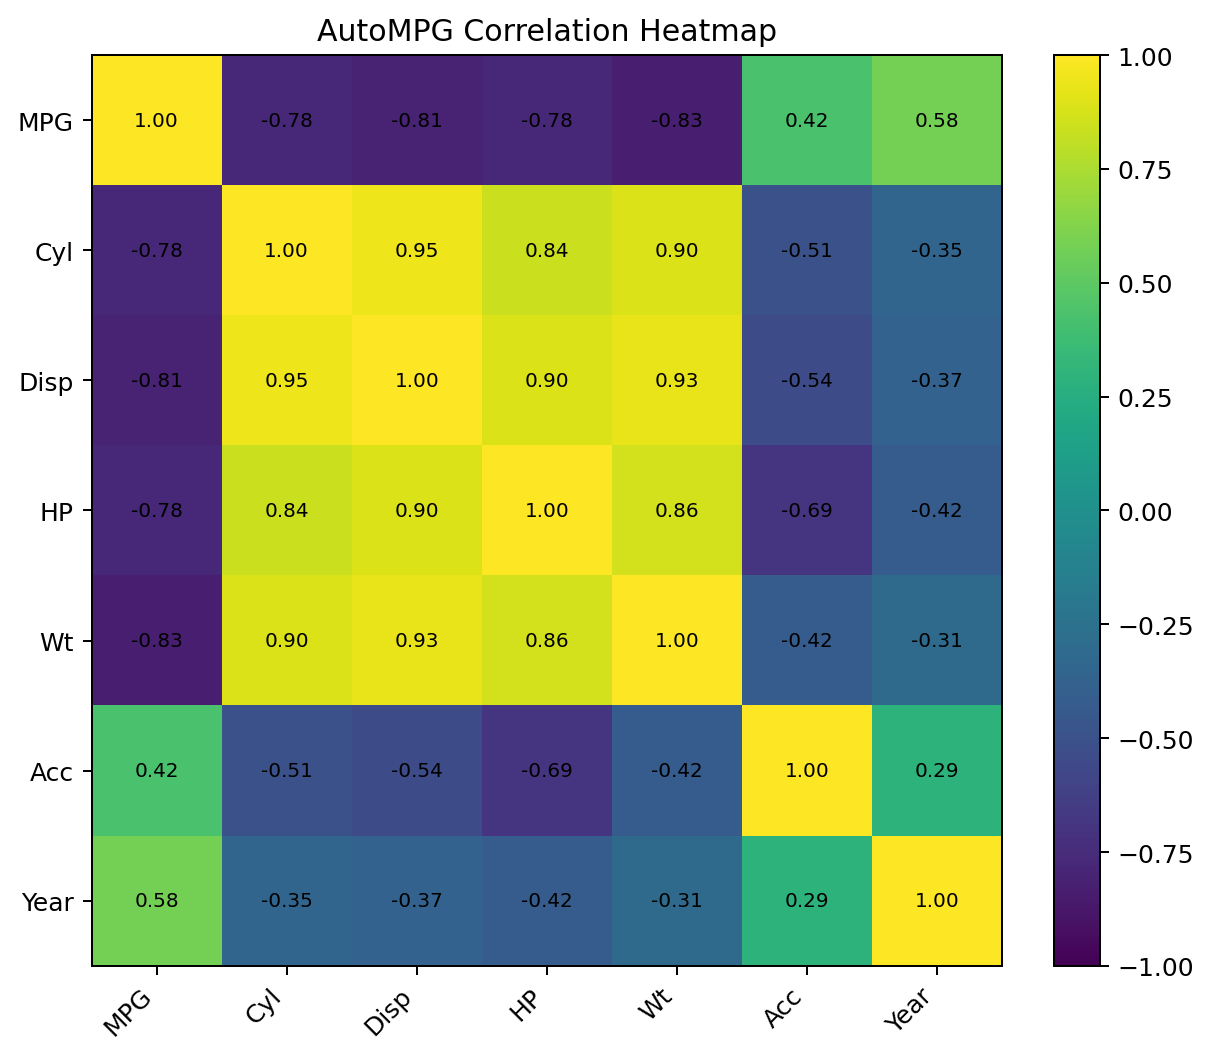
\includegraphics[width=0.78\textwidth]{figures/auto_corr_heatmap.png}
\caption{AutoMPG correlation heatmap. The strongest absolute correlations with
MPG occur for weight and displacement.}
\end{figure}

\subsection{Simple Regression Using Displacement}

Simple linear regression was performed in both Python using
\texttt{statsmodels} and Scala using ScalaTion. The two implementations
produced essentially identical results. The fitted equation was

\[
\widehat{MPG}=35.1206-0.0601(\mathrm{Displacement}).
\]

The negative slope indicates that greater engine displacement is associated
with lower fuel economy. A one-unit increase in displacement is associated
with an estimated decrease of approximately 0.0601 MPG. The slope was
statistically significant ($p<0.001$).

ScalaTion reported $R^2=0.648229$ and adjusted $R^2=0.647327$, consistent
with the \texttt{statsmodels} results. Thus, displacement alone explained
approximately 64.8\% of the observed variation in MPG. ScalaTion also reported
an RMSE of approximately 4.62 MPG.

\begin{figure}[H]
\centering
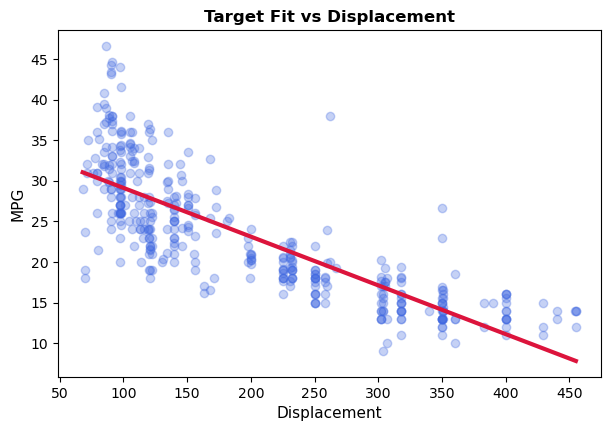
\includegraphics[width=0.78\textwidth]{figures/auto_displacement_fit.png}
\caption{Observed MPG values and fitted simple regression values versus
displacement.}
\end{figure}

\subsection{Simple Regression Using Weight}

The simple regression using vehicle weight also produced nearly identical
results in ScalaTion and \texttt{statsmodels}. The fitted equation was

\[
\widehat{MPG}=46.2165-0.007647(\mathrm{Weight}).
\]

The negative slope indicates that heavier vehicles tend to have lower fuel
economy. A one-unit increase in vehicle weight is associated with an estimated
decrease of approximately 0.00765 MPG. The slope was statistically significant
($p<0.001$).

ScalaTion reported $R^2=0.692630$ and adjusted $R^2=0.691842$, again matching
the \texttt{statsmodels} results. Therefore, vehicle weight alone explained
approximately 69.3\% of the variation in MPG. ScalaTion reported an RMSE of
approximately 4.32 MPG.

\begin{figure}[H]
\centering
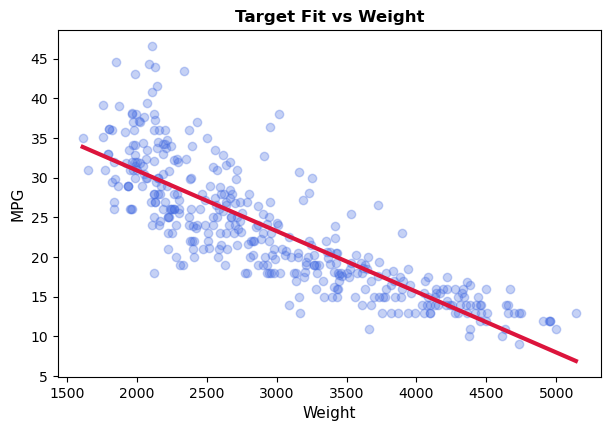
\includegraphics[width=0.78\textwidth]{figures/auto_weight_fit.png}
\caption{Observed MPG values and fitted simple regression values versus
vehicle weight.}
\end{figure}

\subsection{AutoMPG Discussion}

Both selected predictors exhibited strong and statistically significant
negative relationships with MPG, and the ScalaTion and \texttt{statsmodels}
implementations produced essentially identical parameter estimates and
goodness-of-fit measures. Vehicle weight provided the stronger of the two
simple regression models, with $R^2\approx0.693$, compared with
$R^2\approx0.648$ for displacement. This is consistent with the correlation
analysis, in which weight also had the stronger absolute correlation with MPG.

\newpage
\section{Concrete Compressive Strength}

The Concrete Compressive Strength dataset contains 1,030 observations, eight
predictors, and one response variable. The response is concrete compressive
strength, measured in megapascals (MPa).

\subsection{Preprocessing}

All nine variables were numeric, so no string-valued columns required removal
or encoding. No missing values were identified, and therefore no imputation or
row removal was required.

Potential outliers were evaluated with boxplots and the $1.5\times IQR$ rule.
The analysis identified 2 potential outliers for blast furnace slag, 9 for
water, 10 for superplasticizer, 5 for fine aggregate, 59 for age, and 4 for
compressive strength. Cement, fly ash, and coarse aggregate had no IQR
outliers. The flagged observations were retained because the IQR criterion
identifies unusual values but does not establish that those values are
incorrect. In particular, large age values may correspond to valid longer
curing periods.

\subsection{Statistical Summary}

\begin{table}[H]
\centering
\caption{Concrete descriptive statistics.}
\label{tab:concrete-summary}
\resizebox{\textwidth}{!}{
\begin{tabular}{lrrrrrrrr}
\toprule
Variable & Count & Mean & SD & Min & Q1 & Median & Q3 & Max \\
\midrule
Cement & 1030 & 281.168 & 104.506 & 102.00 & 192.375 & 272.900 & 350.000 & 540.0 \\
Blast Furnace Slag & 1030 & 73.896 & 86.279 & 0.00 & 0.000 & 22.000 & 142.950 & 359.4 \\
Fly Ash & 1030 & 54.188 & 63.997 & 0.00 & 0.000 & 0.000 & 118.300 & 200.1 \\
Water & 1030 & 181.567 & 21.354 & 121.80 & 164.900 & 185.000 & 192.000 & 247.0 \\
Superplasticizer & 1030 & 6.205 & 5.974 & 0.00 & 0.000 & 6.400 & 10.200 & 32.2 \\
Coarse Aggregate & 1030 & 972.919 & 77.754 & 801.00 & 932.000 & 968.000 & 1029.400 & 1145.0 \\
Fine Aggregate & 1030 & 773.580 & 80.176 & 594.00 & 730.950 & 779.500 & 824.000 & 992.6 \\
Age & 1030 & 45.662 & 63.170 & 1.00 & 7.000 & 28.000 & 56.000 & 365.0 \\
Compressive Strength & 1030 & 35.818 & 16.706 & 2.33 & 23.710 & 34.445 & 46.135 & 82.6 \\
\bottomrule
\end{tabular}}
\end{table}

Several variables show evidence of skewness, particularly blast furnace slag,
fly ash, superplasticizer, and age, as reflected by differences between their
means and medians.

\subsection{Correlation Analysis and Predictor Selection}

Cement had the strongest absolute correlation with compressive strength
($r=0.498$), followed by superplasticizer ($r=0.366$). These variables were
selected for the two simple regression analyses.

\begin{table}[H]
\centering
\caption{Concrete Pearson correlation matrix.}
\label{tab:concrete-corr}
\resizebox{\textwidth}{!}{
\begin{tabular}{lrrrrrrrrr}
\toprule
 & Cem & Slag & Ash & Water & SP & Coarse & Fine & Age & Strength \\
\midrule
Cem      & 1.000 & -0.275 & -0.397 & -0.082 & 0.092 & -0.109 & -0.223 & 0.082 & 0.498 \\
Slag     & -0.275 & 1.000 & -0.324 & 0.107 & 0.043 & -0.284 & -0.282 & -0.044 & 0.135 \\
Ash      & -0.397 & -0.324 & 1.000 & -0.257 & 0.378 & -0.010 & 0.079 & -0.154 & -0.106 \\
Water    & -0.082 & 0.107 & -0.257 & 1.000 & -0.658 & -0.182 & -0.451 & 0.278 & -0.290 \\
SP       & 0.092 & 0.043 & 0.378 & -0.658 & 1.000 & -0.266 & 0.223 & -0.193 & 0.366 \\
Coarse   & -0.109 & -0.284 & -0.010 & -0.182 & -0.266 & 1.000 & -0.178 & -0.003 & -0.165 \\
Fine     & -0.223 & -0.282 & 0.079 & -0.451 & 0.223 & -0.178 & 1.000 & -0.156 & -0.167 \\
Age      & 0.082 & -0.044 & -0.154 & 0.278 & -0.193 & -0.003 & -0.156 & 1.000 & 0.329 \\
Strength & 0.498 & 0.135 & -0.106 & -0.290 & 0.366 & -0.165 & -0.167 & 0.329 & 1.000 \\
\bottomrule
\end{tabular}}
\end{table}

\begin{figure}[H]
\centering
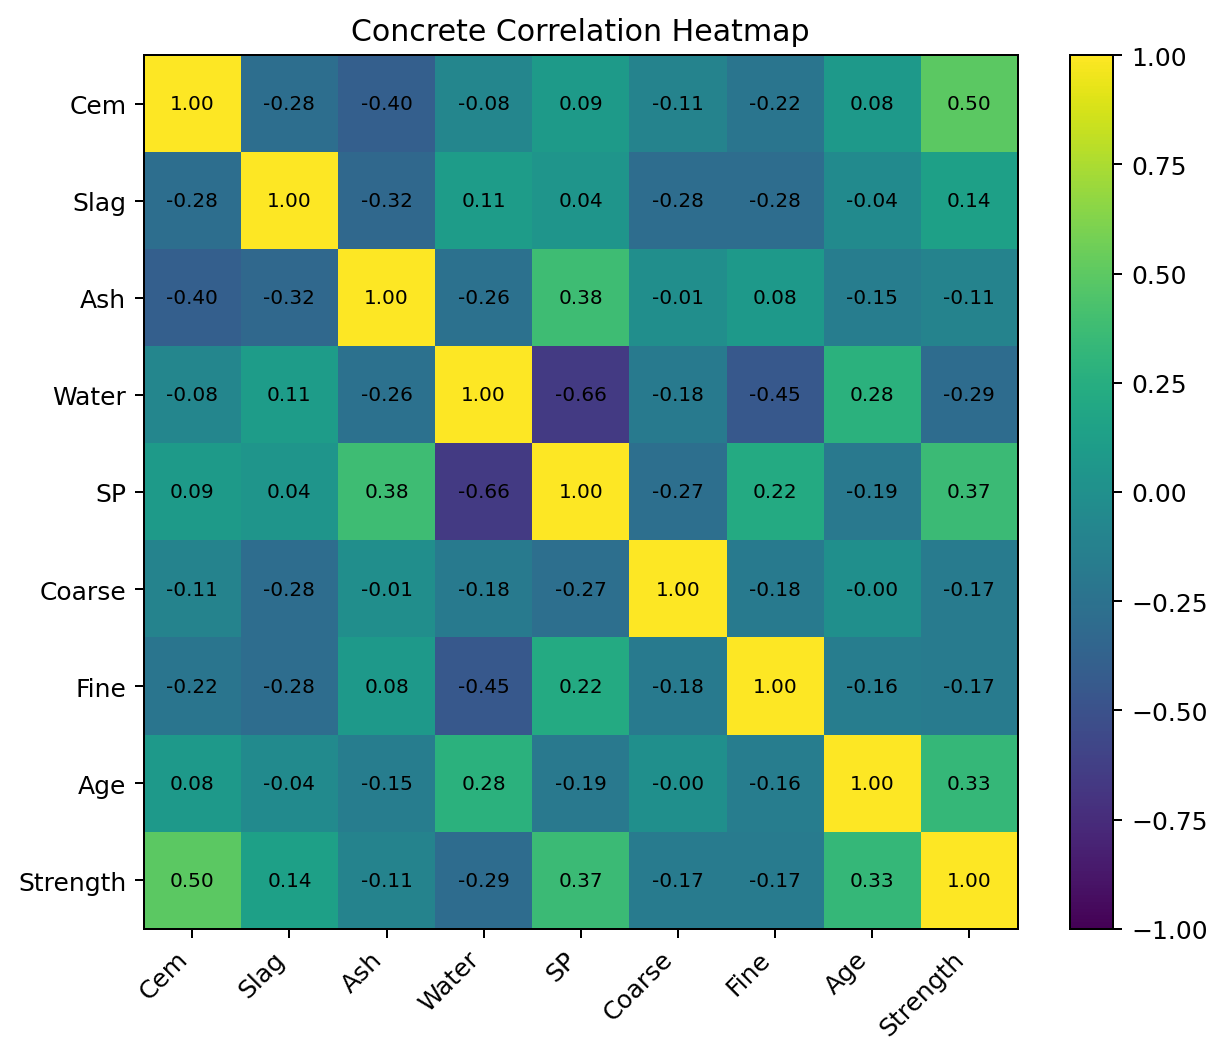
\includegraphics[width=0.82\textwidth]{figures/concrete_corr_heatmap.png}
\caption{Concrete correlation heatmap. Cement and superplasticizer have the
strongest absolute correlations with compressive strength.}
\end{figure}

\subsection{Simple Regression Using Cement}

Simple linear regression was performed using both Python's
\texttt{statsmodels} package and ScalaTion. Both implementations produced
essentially identical coefficient estimates. The fitted model was

\[
\widehat{\mathrm{Strength}}
=
13.4425+0.07958(\mathrm{Cement}),
\]

where cement content is measured in kg/m$^3$ and compressive strength is
measured in MPa.

A 1 kg/m$^3$ increase in cement content is associated with an estimated
increase of approximately 0.0796 MPa in compressive strength. The slope was
statistically significant ($p<0.001$). ScalaTion reported $R^2=0.247837$ and
adjusted $R^2=0.247105$, consistent with the \texttt{statsmodels} results.
Cement alone therefore explained approximately 24.8\% of the observed
variation in compressive strength. ScalaTion reported an RMSE of approximately
14.48 MPa.

\IfFileExists{figures/concrete_cement_fit.png}{
\begin{figure}[H]
\centering

\includegraphics[width=0.78\textwidth]{figures/concrete_cement_fit.png}
\caption{Observed and fitted compressive strength values versus cement.}
\end{figure}
}{
\begin{figure}[H]
\centering
\fbox{\parbox{0.82\textwidth}{\centering
\textbf{Figure still required:} export the observed-versus-fitted plot for
Cement and save it as \texttt{figures/concrete\_cement\_fit.png}.}}
\caption{Placeholder for the required Cement observed-versus-fitted plot.}
\end{figure}
}

\subsection{Simple Regression Using Superplasticizer}

The simple regression using superplasticizer produced essentially identical
results in ScalaTion and \texttt{statsmodels}. The fitted equation was

\[
\widehat{\mathrm{Strength}}
=
29.4660+1.02373(\mathrm{Superplasticizer}),
\]

where superplasticizer content is measured in kg/m$^3$.

A 1 kg/m$^3$ increase in superplasticizer content is associated with an
estimated increase of approximately 1.024 MPa in compressive strength. The
slope was statistically significant ($p<0.001$). ScalaTion reported
$R^2=0.134014$ and adjusted $R^2=0.133171$, matching the
\texttt{statsmodels} results to rounding precision. Superplasticizer alone
explained approximately 13.4\% of the observed variation in compressive
strength. ScalaTion reported an RMSE of approximately 15.54 MPa.

\IfFileExists{figures/concrete_superplasticizer_fit.png}{
\begin{figure}[H]
\centering
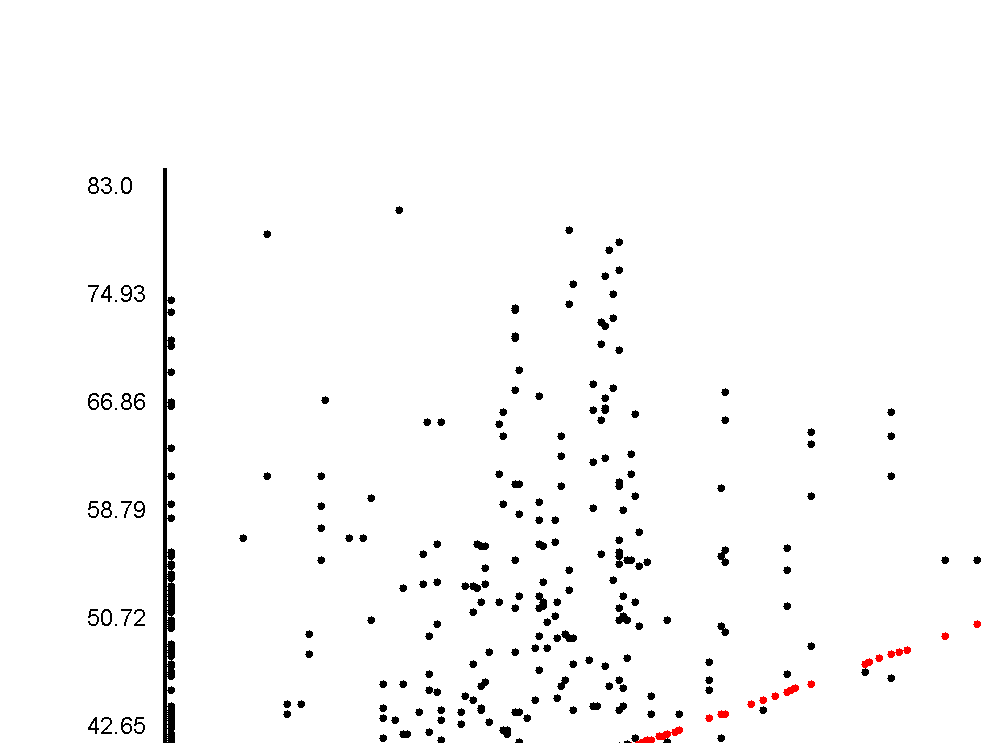
\includegraphics[width=0.78\textwidth]{figures/concrete_superplasticizer_fit.png}
\caption{Observed and fitted compressive strength values versus
superplasticizer.}
\end{figure}
}{
\begin{figure}[H]
\centering
\fbox{\parbox{0.82\textwidth}{\centering
\textbf{Figure still required:} export the observed-versus-fitted plot for
Superplasticizer and save it as
\texttt{figures/concrete\_superplasticizer\_fit.png}.}}
\caption{Placeholder for the required Superplasticizer observed-versus-fitted
plot.}
\end{figure}
}

\subsection{Concrete Discussion}

Both selected predictors exhibited positive and statistically significant
linear relationships with concrete compressive strength, and ScalaTion and
\texttt{statsmodels} produced essentially identical results. Cement provided
the stronger simple regression model, with $R^2\approx0.248$, compared with
$R^2\approx0.134$ for superplasticizer. This ordering is consistent with the
correlation analysis. However, neither predictor individually explained the
majority of the variation in strength, indicating that compressive strength
depends on multiple mixture components and curing conditions.

\newpage
\section{Airfoil Self-Noise}

The Airfoil Self-Noise dataset contains 1,503 observations, five predictor
variables, and the response variable scaled sound pressure level in dB.

\subsection{Preprocessing}

All six original dataset variables were numeric and no missing values were
detected. Therefore, no string encoding, imputation, or row deletion was
required.

The $1.5\times IQR$ rule identified 86 potential outliers for frequency, 30
for angle of attack, 124 for displacement thickness, and 4 for sound pressure
level. No IQR outliers were identified for chord length or free-stream
velocity. These observations were retained because the IQR rule identifies
statistically unusual observations but does not show that the observations are
incorrect. Removing valid observations could discard information from less
common experimental conditions.

The notebook had also retained a generated prediction column named
\texttt{y\_hat} in some saved outputs because cells had been executed out of
order. Since \texttt{y\_hat} is not an original Airfoil variable, it is
excluded from the statistical summary and correlation analysis in this report.

\subsection{Statistical Summary}

\begin{table}[H]
\centering
\caption{Airfoil Self-Noise descriptive statistics.}
\label{tab:airfoil-summary}
\resizebox{\textwidth}{!}{
\begin{tabular}{lrrrrrrrr}
\toprule
Variable & Count & Mean & SD & Min & Q1 & Median & Q3 & Max \\
\midrule
Frequency & 1503 & 2886.381 & 3152.573 & 200.000 & 800.000 & 1600.000 & 4000.000 & 20000.000 \\
Angle of Attack & 1503 & 6.782 & 5.918 & 0.000 & 2.000 & 5.400 & 9.900 & 22.200 \\
Chord Length & 1503 & 0.137 & 0.094 & 0.025 & 0.051 & 0.102 & 0.229 & 0.305 \\
Free-Stream Velocity & 1503 & 50.861 & 15.573 & 31.700 & 39.600 & 39.600 & 71.300 & 71.300 \\
Displacement Thickness & 1503 & 0.011 & 0.013 & 0.000 & 0.003 & 0.005 & 0.016 & 0.058 \\
Sound Pressure Level & 1503 & 124.836 & 6.899 & 103.380 & 120.191 & 125.721 & 129.996 & 140.987 \\
\bottomrule
\end{tabular}}
\end{table}

Sound pressure level has a mean of 124.836 dB and a standard deviation of
6.899 dB. Frequency spans a particularly large range, from 200 Hz to 20,000
Hz.

\subsection{Correlation Analysis and Predictor Selection}

Frequency has the strongest absolute correlation with sound pressure level
($r=-0.391$), followed by displacement thickness ($r=-0.313$). These two
predictors were therefore selected for simple regression.

\begin{table}[H]
\centering
\caption{Airfoil Self-Noise Pearson correlation matrix.}
\label{tab:airfoil-corr}
\resizebox{\textwidth}{!}{
\begin{tabular}{lrrrrrr}
\toprule
 & Freq & AoA & Chord & Vel & Thick & SPL \\
\midrule
Freq  & 1.000 & -0.273 & -0.004 & 0.134 & -0.230 & -0.391 \\
AoA   & -0.273 & 1.000 & -0.505 & 0.059 & 0.753 & -0.156 \\
Chord & -0.004 & -0.505 & 1.000 & 0.004 & -0.221 & -0.236 \\
Vel   & 0.134 & 0.059 & 0.004 & 1.000 & -0.004 & 0.125 \\
Thick & -0.230 & 0.753 & -0.221 & -0.004 & 1.000 & -0.313 \\
SPL   & -0.391 & -0.156 & -0.236 & 0.125 & -0.313 & 1.000 \\
\bottomrule
\end{tabular}}
\end{table}

\begin{figure}[H]
\centering
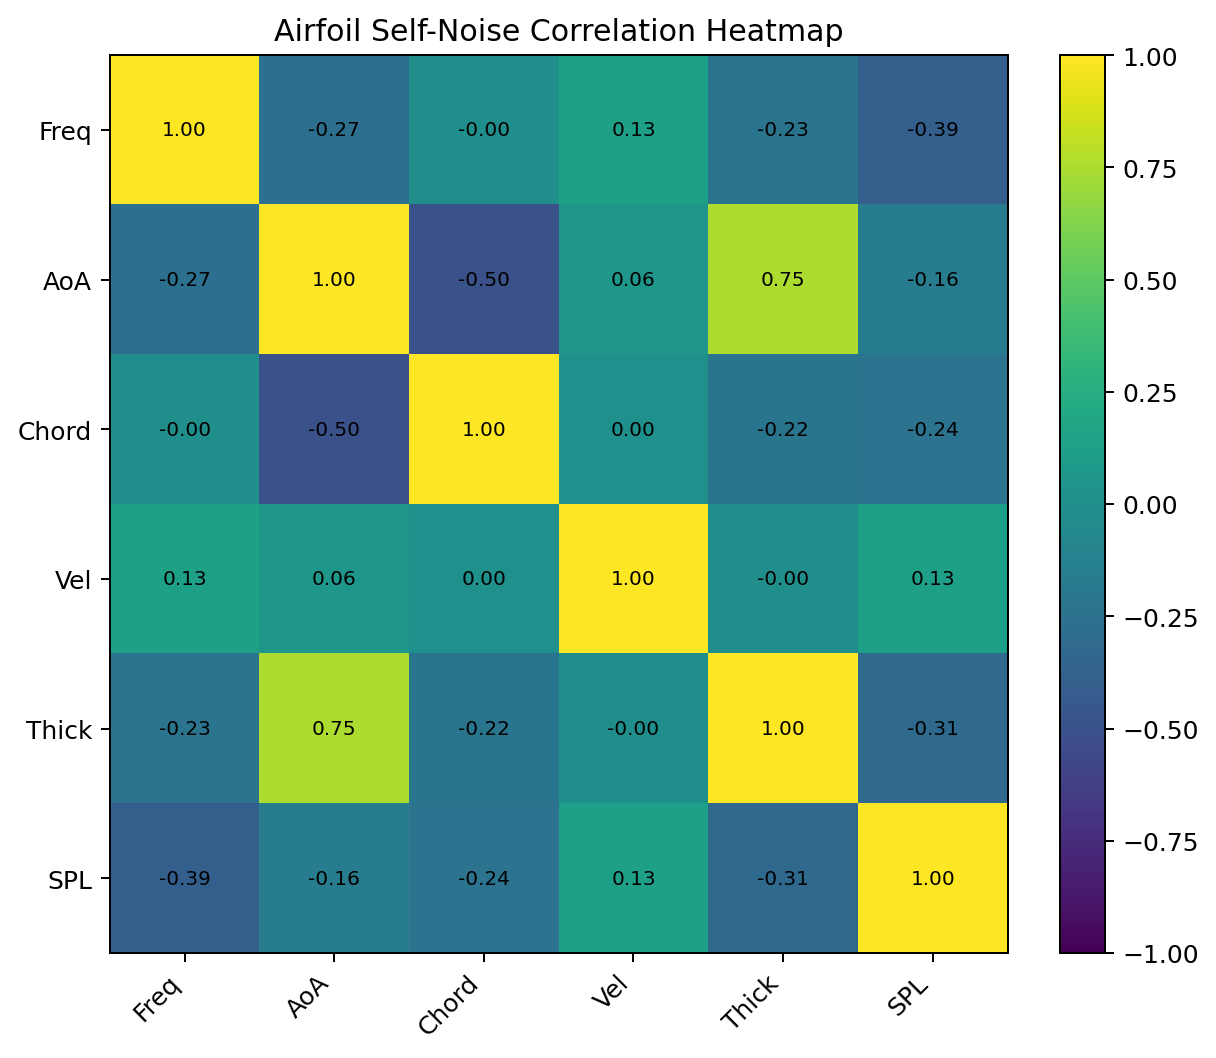
\includegraphics[width=0.78\textwidth]{figures/airfoil_corr_heatmap.png}
\caption{Airfoil Self-Noise correlation heatmap after excluding the generated
\texttt{y\_hat} column.}
\end{figure}

\subsection{Simple Regression Using Frequency}

Both software implementations produced essentially identical coefficient
estimates. The fitted model was

\[
\widehat{\mathrm{SPL}}
=
127.3037-0.000855(\mathrm{Frequency}).
\]

The negative slope indicates an inverse association between frequency and
sound pressure level. An increase of 1,000 Hz is associated with an estimated
decrease of approximately 0.855 dB in sound pressure level. The slope was
statistically significant ($p<0.001$).

ScalaTion reported $R^2=0.152655$ and adjusted $R^2=0.152091$, which agreed
with the corresponding \texttt{statsmodels} results. Thus, frequency alone
explained approximately 15.3\% of the observed variability in sound pressure
level.

\begin{figure}[H]
\centering
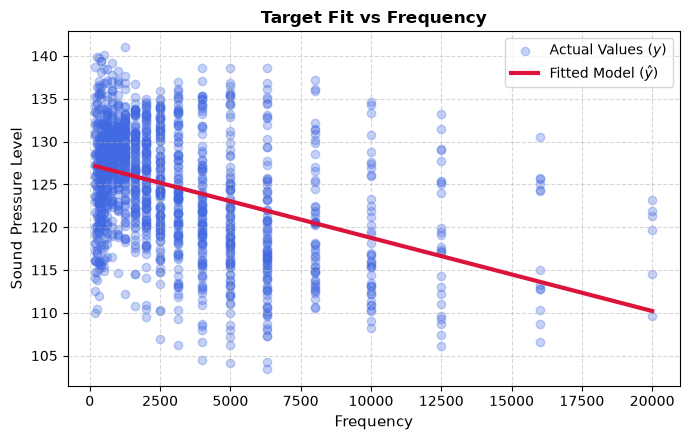
\includegraphics[width=0.78\textwidth]{figures/airfoil_frequency_fit.png}
\caption{Observed sound pressure levels and fitted values versus frequency.}
\end{figure}

\subsection{Simple Regression Using Displacement Thickness}

The fitted equation was

\[
\widehat{\mathrm{SPL}}
=
126.6632-164.0275(\mathrm{Displacement\ Thickness}),
\]

where displacement thickness is measured in meters.

The slope of $-164.0275$ dB per meter is equivalent to approximately
$-0.164$ dB per millimeter. Therefore, a 1 mm increase in displacement
thickness is associated with an estimated decrease of approximately 0.164 dB
in sound pressure level. The coefficient was statistically significant
($p<0.001$).

ScalaTion reported $R^2=0.097762$ and adjusted $R^2=0.097161$, again matching
the \texttt{statsmodels} results to rounding precision. Displacement thickness
alone therefore explained approximately 9.8\% of the observed variability in
sound pressure level.

\begin{figure}[H]
\centering
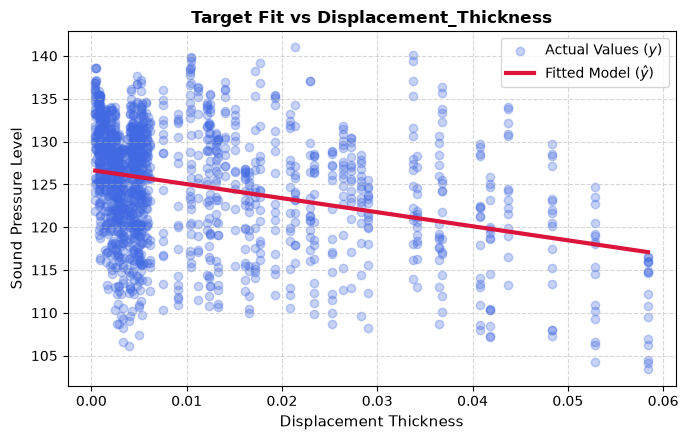
\includegraphics[width=0.78\textwidth]{figures/airfoil_displacement_fit.png}
\caption{Observed sound pressure levels and fitted values versus displacement
thickness.}
\end{figure}

\subsection{Airfoil Discussion}

Both selected predictors had statistically significant negative relationships
with sound pressure level, and both software packages produced essentially
identical results. Frequency provided the stronger simple regression model,
with $R^2\approx0.153$ compared with approximately 0.098 for displacement
thickness. Nevertheless, neither predictor explains a large proportion of the
response variability by itself, suggesting that sound pressure level is
influenced by additional experimental variables.

\newpage
\section{Overall Conclusion}

Across all three datasets, the predictors selected from the correlation
analysis were used consistently in both software implementations. ScalaTion
and \texttt{statsmodels} produced essentially identical fitted coefficients
and goodness-of-fit values for the six simple regression relationships.

The strongest individual simple regression among the analyses was vehicle
weight for AutoMPG, which explained approximately 69.3\% of MPG variation.
The Concrete and Airfoil models had lower $R^2$ values, indicating that their
responses are less adequately explained by one predictor at a time. The
results illustrate both the usefulness and the limitations of simple linear
regression: a statistically significant relationship may exist even when a
single predictor leaves substantial response variation unexplained.

\end{document}
